\chapter{序論}
\label{chap_intro}

\section{研究背景}
がん検診では見落としなく病変を見つけることが求められているため,担当医が判定してから専門医がダブルチェックをしている.現在の日本の病理の専門医は2483名\cite{pathology}で,その人数に対して標本500万件を年間で処理している現状である.

従来の内視鏡の生検は食道,大腸,小腸,胃などを鉗子で2 mm角程度の立方体で抜き出し,染色したものを2,3断面にカットしてから病理診断医が顕微鏡で観察し,腫瘍か非腫瘍かを判別したり,その悪性度を判定している.しかし,断面のみの観察では内部に腫瘍がある場合に見落としてしまうリスクがある.そこで組織透明化技術(LUCID-A)\cite{sekitani2016ultraflexible}を用いて内視鏡検体を透明化して丸ごと観察する.\fig{lucid}はマウス小腸をLUCID-Aで透明化処理し,二光子励起顕微鏡で撮影した像である.従来の透明化技術では時間が経つと検体が損傷してしまい,医療法第24条診療録の記載及び保存の二項と療養担当規則9条に規定されている5年間の保存義務を満たせなかった.しかし,LUCID-Aは5年を超える長期保存が可能であり,水に浸すと元に戻りかつ毒性もないため,生検と相性が良い.

現在でも専門医の負担は大きいと言えるが,透明化技術で全断面を観察可能となれば,その全てを専門医が診断することになり現実的ではない.
そこで,人工知能を用いて腫瘍と推測されるような検体のスクリーニングを行って専門医の確認が必要な症例を絞り込んで診断することが必要である.

\begin{figure}[H]
	\centering
	\begin{minipage}[b]{0.4\columnwidth}
		\centering
		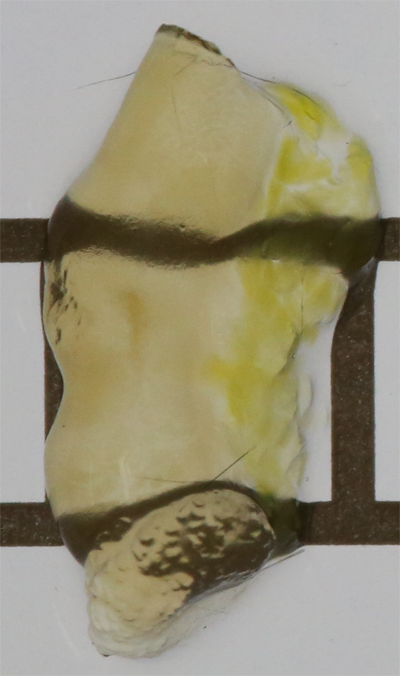
\includegraphics[clip, angle=90, width=\linewidth]{fig/chapter1/colon_lucid}
		\subcaption{Trasparent intestine}
	\end{minipage}
	\begin{minipage}[b]{0.4\columnwidth}
		\centering
		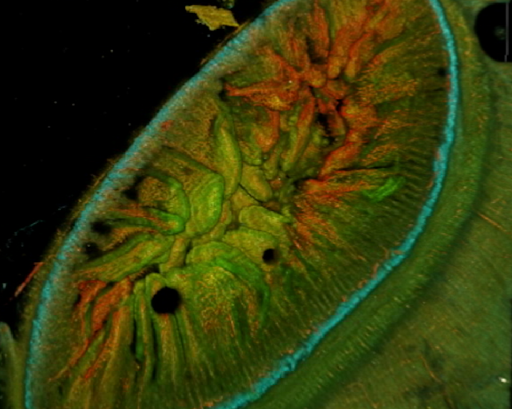
\includegraphics[clip, width=\linewidth]{fig/chapter1/colon_microscope}
		\subcaption{Image taken by microscope}
	\end{minipage}
	\caption{Transparent specimen}
	\label{fig:lucid}
\end{figure}


\section{先行研究}\label{sec:先行研究}
人工知能に関する研究は現在盛んに行われている\cite{lecun2015deep, hoo2016deep}.特に画像認識の分野では,ILSVRC2012という画像認識の大会でこれまでは少しずつ改良を続けてきたところを,Hintonらが深層学習を利用することで一気に画像認識の精度を高めるという衝撃を与えた\cite{AlexNet}.その後は深層学習を用いたモデルが主流となり,現在では95\%以上の認識率を超え人間よりも高い認識精度を達成している\cite{ResNet}.

この画像認識の技術を医療画像に応用する研究が行われている\cite{inglese2017deep, hoo2016deep, havaei2017brain}.深層学習を用いた医療画像の診断アルゴリズムの先行研究としては,乳がん\cite{wang2016deep}の検体や皮膚がん\cite{esteva2017dermatologist}の検体などがある.これらの検体の認識では,専門医と同程度の精度を達成している.

しかしこのように高い精度を出すためには,数万枚の画像データを用意する必要があることに加えて,その画像を認識する目的のカテゴリーに分類する作業(アノテーション)が必要がある.
少量の画像データしか用意できないと,いくつかの問題が生じる.まず,様々なバリエーションに対応することができなくなる.また,深層学習の訓練に用いるデータが医師によってばらつきがある場合は,教師データを作成した医師の判断が大きく反映されてしまうという問題が生じる.これらの問題があるため医療画像における深層学習を用いた診断システムは,大量にデータを用意するまでの時間や人的コストを大きく払うことになっているのが現状である.

一方,病理画像の見落とし防止のために3次元画像を取得して解析する研究が行われている.先行研究としては,CT\cite{dou20163d}やMRI\cite{fmri}画像の解析が上げられる.CTやMRIの場合は,画像の分解能が顕微鏡像よりも低く,深さ方向にも1ステップ数mmオーダーで1検体あたり取れる深さ像は30枚程度である.そのため2次元画像の深層学習による解析を3次元にそのまま拡張して解析することができ,見落としを防止する診断のアルゴリズムを作ることができている.しかし,本研究のように深さ方向に数100ステップある画像を解析することは,深層学習の訓練に使うパラメータが大きくなり過ぎて学習が安定しないという問題がある.


\section{本研究の目的}
本研究の目的は,内視鏡生検検体を透明にし,深層学習を利用して腫瘍を見落とさない診断アルゴリズムを開発することである.組織透明化技術LUCID-Aを用いて検体を丸ごと透明化し,共焦点レーザー顕微鏡で観察することで検体の内部まで3次元情報として解析することができる.

\begin{figure}[H]
	\centering
	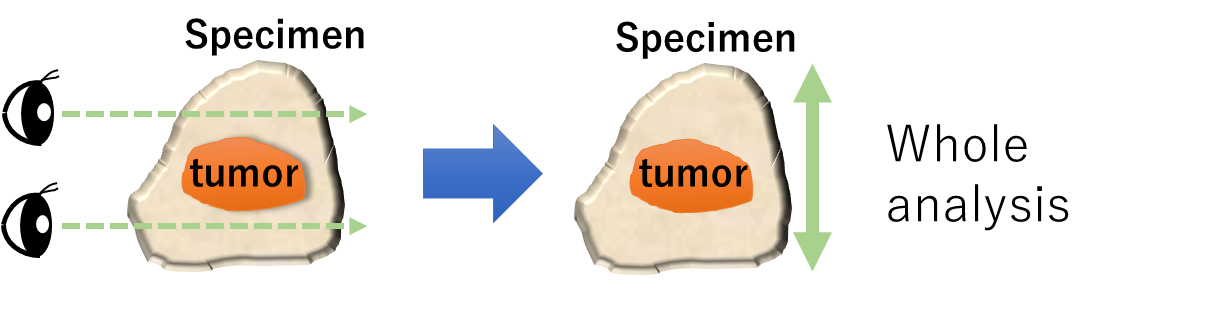
\includegraphics[width=0.9\linewidth]{fig/chapter1/whole_image_analysis}
	\caption{Schematic of whole image analysis}
	\label{fig:wholeimageanalysis}
\end{figure}

透明化されたサンプルを共焦点レーザー顕微鏡で撮影すると,従来のカットする手法に換算して〜500断面に相当する.そのため,得られる顕微鏡撮影像が従来の2,3カットに対して数100倍となるので,専門医が診断をする負担が大きくなってしまう.そこで,人工知能(Artificial Intelligence: AI)が3次元画像を解析して病変を検知し,専門医に提示することで病変の見落としリスク(偽陰性)がゼロになる診断支援システムを開発した.

\section{構成}
本研究では,以下の4つのことを行った.

\subsection*{色空間変換}
内視鏡の検体はDAPIで染色して共焦点レーザー顕微鏡で撮影している.そのため,従来の染色法であるHE染色と同じ色空間に変換することで,病理医が見慣れた画像にして見やすくなるだけでなく,HE画像データベースを活用した転移学習を可能にした.

\subsection*{3次元画像解析}
生検検体の3次元画像を解析することで,2次元画像では判断の難しいものを3次元特有の情報を用いることで判定精度を上げた.本研究で用いる透明化処理した検体は共焦点レーザー顕微鏡で撮影するため分解能が高く,深さ方向にも1ステップ数$\upmu$mオーダーで400〜700枚が撮影することができる.このように深さ方向にも分解能が高い3次元画像においても,特徴を抽出できるような解析手法を研究した.

\subsection*{半教師あり学習}
深層学習で解析を行う場合はデータを大量に準備する必要がある.今回のように,新しい撮影手法であったり,希少な病気であったりすると医療データを数多く集められないことがある.\ref{sec:先行研究}節で述べたように,少ない教師データで識別精度を上げることは深層学習において困難とされている.

画像の構造的な特徴のパターンを学ぶ教師なし学習と呼ばれる手法では,教師ラベルを必要とせず画像データがあれば良い.この教師なし学習と教師ラベルを使った学習を組み合わせた,半教師あり学習(弱教師あり学習とも呼ばれる)によって病理画像が正常から異常になる過程には連続的な性質があることを活用して正常と異常の分布を学習し,より正常と腫瘍の認識精度を高めることに取り組んだ.

\subsection*{腫瘍検出結果の可視化}
最後に,この深層学習による腫瘍の検出結果を医師が診断する際のサポートになるように可視化することに取り組んだ.深層学習は判断の理由が分からないためブラックボックスと呼ばれ,信頼性が求められる場面では利用に対して不安視されることがある.そのため腫瘍と正常の診断の判断の理由を可視化する必要がある.
明らかに正常のものと,腫瘍かもしれない領域で区別して,腫瘍かもしれない部分を医師に提示することで腫瘍を見落とさないような医師の負担を減らすためのスクリーニングとして利用するため可視化処理を行う.

